\chapter{Spinning Switches}
\label{cha:research_topic_1}

What this paper does:
\begin{enumerate}
  \item Generalizes switches to arbitrary groups.
  \item Proves a result when switches look like $p$-groups.
  \item Finds the ``correct'' model: the wreath products.
  \item Provides reductions for when strategies don't exist, which are easy to prove with the wreath product model.
  \item Comes up with an example where something isn't a prime power. ($S_3 \wr C_2$ is nontrivial. Of course $G \wr \mathbf{1}$ also works.)
\end{enumerate}

\section{TODO}
\begin{enumerate}
  \item Provide solution to Winkler puzzle.
  \item Fill out Example \ref{ex:NoSolutionZ2C3}.
  \item Incorporate Section \ref{sec:HistoricalProgress} into earlier sections.
  \item Provide example for first reduction. (Theorem \ref{thm:SwitchReduction})
  \item Give other part of example for second reduction. (Theorem \ref{thm:SpinReduction})
  \item Example for third reduction. (Theorem \ref{thm:SpinReduction2})
  \item Define/discuss minimal switching strategies?
  \item Mention conjecture that most groups are $2$-groups
  \item Infinite switching strategy?
    $\mathbb{Z} \wr C_2$ or $\mathbb{Z}_2^\infty \wr C_2$. \\
    (By $\mathbb{Z}_2^\infty$, I mean something isomorphic to the integers under
    XOR: $(\mathbb{Z}, \oplus)$.)
\end{enumerate}

\section{Overview and Preliminaries}
This section provides a brief history of the problem and provides the idea for the more general context.
Section \ref{sec:WreathModel} models these generalizations in the context of the wreath product.
Section \ref{sec:HistoricalProgress} is where all of the references are. [TODO: put this section elsewhere]
Section \ref{sec:Reductions} allows us to prove when Player B does not have a winning strategy.
Section \ref{sec:pGroupStrategy} allows us to make a statement about games that have a prime number of possible moves.
Section \ref{sec:OtherSwitchingStrategies} gives us an example of new kinds of puzzles that have solutions.
Section \ref{sec:OpenQuestions} gives us an example of new kinds of puzzles that have solutions.

\subsection{History}
A closely related puzzle was popularized by Martin Gardner in the
February 1979 edition of his column ``Mathematical Games.'' \cite{Gardner1979Problem}
He wrote that he learned of the puzzle from Robert Tappay of Toronto who
``believes it comes from the U.S.S.R.''

The version under consideration in this paper is first hinted at in 1993
by Yehuda and collaborators \cite{Yehuda1993}.
Ehrenborg and Skinner consider something very similar, which they call the
"Blind Bartender with Boxing Gloves" \cite{Ehrenborg1995}.
This was re-popularized in 2019 when it appeared in ``The Riddler'' from
FiveThirtyEight \cite{FiveThirtyEight}.
Sidana \cite{Sidana2020} provides a detailed overview of the history of this
and related problems.

My preferred version appears in Peter Winkler's 2004 book
\textit{Mathematical Puzzles A Connoisseur's Collection}
\begin{quote}
  Four identical, unlabeled switches are wired in series to a light bulb.
  The switches are simple buttons whose state cannot be directly observed,
  but can be changed by pushing; they are mounted on the corners of a
  rotatable square. At any point, you may push, simultaneously, any subset
  of the buttons, but then an adversary spins the square. Show that there
  is a deterministic algorithm that will enable you to turn on the bulb in
  at most some fixed number of steps. \cite{Winkler2004}
\end{quote}

\subsection{Generalizing Switches}
``The problem can also be generalized by replacing glasses with objects that
have more than two positions. Hence the rotating table leads into deep
combinatorial questions that as far as I know have not yet been explored.''
\cite{Gardner1979Solution}

Two kinds of switches are considered by Yehuda, Etzionn, and Moran in 1993
\cite{Yehuda1993}: switches with a single ``on'' position that behave like
$n$-state roulettes ($\mathbb Z_n$) and switches that behave like
the finite field $\mathbb F_q$.
Yuri Rabinovich \cite{Rabinovich2022} goes further by considering collections
of switches that behave like arbitrary finite dimensional vector spaces over
finite fields.
We can generalize this notion further by considering
switches that behave like arbitrary finite groups.

For example, one could imagine a switch that behaves like the symmetric
group $S_3$, consisting of three identical-looking parts that need to be
arranged in a particular order in order for the switch to be on,
as illustrated in Figure \ref{fig:S3Switch}.

Groups are a useful model for switches because they share many properties of a
desirable switch \begin{enumerate}
  \item Closure. Every change we make to a switch leaves it in a valid state.
  \item Identity. We can ``do nothing'' to a switch and leave it in whatever
    state it is in.
  \item Inverses. No matter what state a switch is in, we can move it to the
    on state.
  \item Associativity. This is not strictly necessary, but it allows us to
    model things better.
    (In Subsection \ref{sub:quasigroupSwitches}, we briefly discuss dropping
    this assumption by considering switches that behave like quasigroups with
    identity.)
\end{enumerate}

% In a similar vein, we could construct a switch that behaves like the dihedral
% group of the square. Perhaps the switch is a thin square prism that fits into a
% square slot in such a way that only one orientation of the prism completes the
% circuit. See Figure \ref{fig:D8Switch} for a simple schematic.
% [A schematic for a switch that looks like $D_4$.]
% Or one could imagine a switch that behaves like the dihedral group of the square,
% $D_8$ where the square has a single, unique orientation that completes the circuit.
% Or abstractly, one could think of each switch as an abstract group element,
% where Player B can multiply by anything they like.

\begin{figure}
\center{
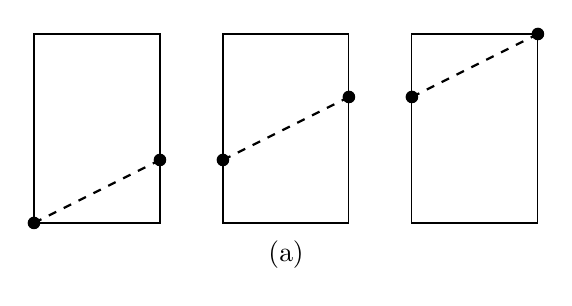
\begin{tikzpicture}[scale=0.8]
  \draw (0,0) rectangle ++(2,3);
  \draw[dashed,thick] (0,0) -- ++(2,1);
  \fill (0,0) circle (0.1);
  \fill (2,1) circle (0.1);

  \draw (3,0) rectangle ++(2,3);
  \draw[dashed,thick] (3,1) -- ++(2,1);
  \fill (3,1) circle (0.1);
  \fill (5,2) circle (0.1);

  \draw (6,0) rectangle ++(2,3);
  \draw[dashed,thick] (6,2) -- ++(2,1);
  \fill (6,2) circle (0.1);
  \fill (8,3) circle (0.1);
  \node at (4, -1/2) {(a)};
\end{tikzpicture}
}

\noindent
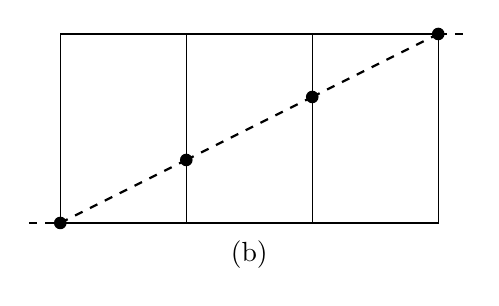
\begin{tikzpicture}[scale=0.8]
  \draw[dashed,thick] (-0.5,0) -- (0,0);
  \fill (0,0) circle (0.1);

  \draw (0,0) rectangle ++(2,3);
  \draw[dashed,thick] (0,0) -- ++(2,1);
  \fill (2,1) circle (0.1);

  \draw (2,0) rectangle ++(2,3);
  \draw[dashed,thick] (2,1) -- ++(2,1);
  \fill (4,2) circle (0.1);

  \draw (4,0) rectangle ++(2,3);
  \draw[dashed,thick] (4,2) -- ++(2,1);
  \fill (6,3) circle (0.1);

  \draw[dashed,thick] (6,3) -- (6.5,3);
  \node at (3, -1/2) {(b)};
\end{tikzpicture}
~
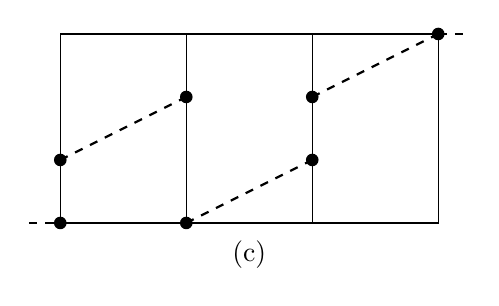
\begin{tikzpicture}[scale=0.8]
  \draw[dashed,thick] (-0.5,0) -- (0,0);
  \fill (0,0) circle (0.1);

  \draw (0,0) rectangle ++(2,3);
  \draw[dashed,thick] (0,1) -- ++(2,1);
  \fill (0,1) circle (0.1);
  \fill (2,2) circle (0.1);

  \draw (2,0) rectangle ++(2,3);
  \draw[dashed,thick] (2,0) -- ++(2,1);
  \fill (2,0) circle (0.1);
  \fill (4,1) circle (0.1);

  \draw (4,0) rectangle ++(2,3);
  \draw[dashed,thick] (4,2) -- ++(2,1);
  \fill (4,2) circle (0.1);
  \fill (6,3) circle (0.1);

  \draw[dashed,thick] (6,3) -- (6.5,3);
  \node at (3, -1/2) {(c)};
\end{tikzpicture}
\caption{
  Part (a) shows a simple schematic for a switch that behaves like $S_3$,
  the symmetric group on three letters.
  The three rectangles can be permuted arbitrarily, but only configuration (b)
  completes the circuit. All other configurations fail to
  complete the circuit (e.g. (c)).
}
\label{fig:S3Switch}
\end{figure}

\subsection{Generalizing Spinning}
We can also consider generalizations of ``spinning'' the switches.
In particular, we will adopt the generalization from
Ehrenborg and Skinner's \cite{Ehrenborg1995} 1995 paper, which use
arbitrary finite group actions to permute the switches.
In particular, they provide a criterion that determines which group actions
yield a winning strategy in the case of a given number of ``ordinary'' switches
(those that behave like $\mathbb Z_2$).
Rabinovich \cite{Rabinovich2022} stretches these results a bit further and
looks at certain group actions on collections of switches that behave like
a finite dimensional vector space over a finite field. We build on this result
in the context of more general switches.

\section{The Wreath Product Model}
\label{sec:WreathModel}
Remind you of the definition of a wreath product, and give examples of how it
models the spinning switches puzzle.
\subsection{Modeling Generalized Spinning Switches Puzzles}
\begin{definition}[\cite{TODORotmanGroupTheoryFIXME}]
  Let $G$ and $H$ be groups,
  let $\Omega$ be a finite $H$-set, and
  let $K = \prod_{\omega \in \Omega} G_\omega$, where $G_\omega \cong G$
  for all $\omega \in \Omega$.
  Then the \textbf{wreath product} of $G$ by $H$ denoted by $G \wr H$,
  is the semidirect product of $K$ by $H$,
  where $H$ acts on $K$ by $h \cdot (d_\omega) = d_{h^{-1}\omega}$ for $g \in H$ and
  $(g_\omega) \in \prod_{\omega \in \Omega} G_\omega$.
  The normal subgroup $K$ of $G \wr H$ is called
  the \textbf{base} of the wreath product.
\end{definition}

The reason this definition is used is because it models the game well, where
$G$ models the behavior of the switches, $\Omega$ models the switches themselves,
and the way $H$ acts on $\Omega$ models the ways the adversary can ``spin'' the
board.

An element of $(k, h) \in G \wr H$ represents a turn of the game:
Player B chooses $k$ to indicate how they want to modify each of their switches
and then Player A chooses $k$ to indicate how they want to permute the switches.

\begin{example}
  Consider the setup in the original version of the problem consisting of
  two-way switches ($\mathbb Z_2$)
  on the corners of a rotating square
  ($C_4 \cong \langle 0^\circ, 90^\circ, 180^\circ, 270^\circ \rangle$).
  This can be modeled as a game on the wreath product $\mathbb Z_2 \wr C_4$.
  We will use the convention that the base of the wreath product, $K$ is
  ordered upper-left, upper-right, lower-right, lower-left, and the group
  action is specified by degrees in the clockwise direction.

  Consider the following two turns:
  \begin{enumerate}
    \item During the first turn,
    Player B toggles the upper-left and lower-right switches, and
    Player A rotates the table $90^\circ$ clockwise.
    This is represented by the element
    $((1,0,1,0), 90^\circ) \in \mathbb Z_2 \wr C_4$.
    \item During the second turn,
    Player B toggles the upper-left switch, and
    Player A rotates the table $90^\circ$ clockwise.
    This is represented by the element
    $((1,0,0,0), 180^\circ) \in \mathbb Z_2 \wr C_4$.
  \end{enumerate}

  As illustrated in Figure \ref{fig:WreathProduct},
  the net result of these two turns is the same as
  a single turn where Player B toggles the upper-left, upper-right, and lower-left
  switches and Player A rotates the board $270^\circ$ clockwise.

  \begin{figure}
    \center
    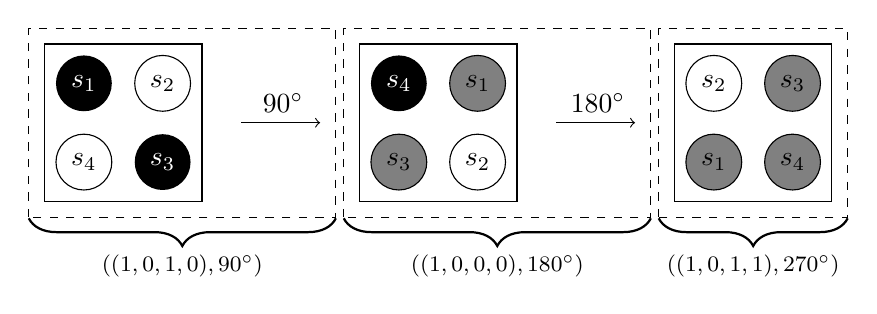
\begin{tikzpicture}
      \draw[dashed] (-0.2,-0.2) rectangle (3.7,2.2);
      \draw [thick,decorate,decoration={brace,amplitude=10pt},yshift=-0.4pt]
        (3.7,-0.2) -- (-0.2,-0.2) node[black,midway,yshift=-0.6cm] {\footnotesize $((1,0,1,0), 90^\circ)$};

      \draw[dashed] (3.8,-0.2) rectangle (7.7,2.2);
      \draw [thick,decorate,decoration={brace,amplitude=10pt},yshift=-0.4pt]
        (7.7,-0.2) -- (3.8,-0.2) node[black,midway,yshift=-0.6cm] {\footnotesize $((1,0,0,0), 180^\circ)$};

      \draw[dashed] (7.8,-0.2) rectangle (10.2,2.2);
      \draw [thick,decorate,decoration={brace,amplitude=10pt},yshift=-0.4pt]
        (10.2,-0.2) -- (7.8,-0.2) node[black,midway,yshift=-0.6cm] {\footnotesize $((1,0,1,1), 270^\circ)$};

      \draw (0,0) rectangle (2,2);
      \node[circle,fill,text=white] at (1/2,3/2) {$s_1$};
      \node[circle,draw] at (3/2,3/2) {$s_2$};
      \node[circle,fill,text=white] at (3/2,1/2) {$s_3$};
      \node[circle,draw] at (1/2,1/2) {$s_4$};
      \draw[->] (2.5,1) -- node[above] {$90^\circ \! \curvearrowright$} (3.5,1) ;

      \draw (4,0) rectangle (6,2);
      \node[circle,fill,text=white] at (9/2,3/2) {$s_4$};
      \node[circle,draw,fill=gray] at (11/2,3/2) {$s_1$};
      \node[circle,draw] at (11/2,1/2) {$s_2$};
      \node[circle,draw,fill=gray] at (9/2,1/2) {$s_3$};

      \draw[->] (6.5,1) -- node[above] {$180^\circ \! \curvearrowright$} (7.5,1) ;

      \draw (8,0) rectangle (10,2);
      \node[circle,draw] at (17/2,3/2) {$s_2$};
      \node[circle,draw,fill=gray] at (19/2,3/2) {$s_3$};
      \node[circle,draw,fill=gray] at (19/2,1/2) {$s_4$};
      \node[circle,draw,fill=gray] at (17/2,1/2) {$s_1$};
    \end{tikzpicture}
    \caption{An illustration of two turns each in the Spinning Switches puzzle,
    modeled as elements of a wreath product.}
    \label{fig:WreathProduct}
  \end{figure}

  The multiplication under the wreath product agrees with this: \begin{align*}
    ((1,0,1,0), 90^\circ) \cdot ((1,0,0,0), 180^\circ)
    &= ((1,0,1,0) + 90^\circ \cdot (1,0,0,0), 90^\circ + 180^\circ) \\
    &= ((1,0,1,1), 270^\circ)
  \end{align*}
\end{example}

Occasionally it is useful to designate a particular state of the switches as the
on state or the winning state, and ordinarily the identity state is the choice
given for this. However, the existence of a winning strategy does not depend on
a particular choice in the winning state; instead, a winning strategy is
equivalent to a choice of moves that will walk over all of the possible
configuration states, regardless of the choice of the adversaries spin.

\subsection{Switching Strategy}

\begin{definition}
  A \textbf{switching strategy} is a finite sequence, $\{k_i \in K\}_{i=1}^N$,
  such that for every sequence ${\{h_i \in H\}_{i=1}^N}$,
  \[
    p(\{e_{G \wr H}, (k_1, h_1), (k_1, h_1)\cdot(k_2, h_2), \cdots, (k_1, h_1)\cdot(k_2, h_2)\cdots(k_N, h_N)\}) = K.
  \]
  where $p \colon G \wr_\Omega H \rightarrow K$ is the projection map from the
  wreath product $G \wr_\Omega H$ onto its base $K$.
\end{definition}

% TODO: Variants of this puzzle require more constraints---if you can only change
% $k$ switches,
% or if all of the switches need only to be in the same state,
% or if you can see the states of the switches and player A rotates after you specify what you want.

This definition is useful because it puts the problem into purely algebraic
terms. It is also useful because it abstracts away the initial state of the
switches: regardless of the initial state $k \in K$, a existence of a switching strategy
means that its inverse $k^{-1} \in K$ appears in the sequence.

\begin{lemma}
  A sequence of moves is guaranteed to ``turn on the lightbulb'' if and only if
  it is a switching strategy.
\end{lemma}
\begin{proof}
  Without loss of generality, say that the ``on'' setting for the switches is
  $\mathrm{id}_K$.
  In the puzzle, we have an initial (hidden) state, $k$.
  Thus, after the $i$-th move, the wreath product
  element that represents the state of the switches is \[
    p\left((k, \mathrm{id}_H)\cdot(k_1, h_1)\cdot(k_2, h_2)\cdots(c_i, h_i)\right)
    = k \cdot p\left((k_1, h_1)\cdot(k_2, h_2)\cdots(c_i, h_i)\right),
  \] by associativity, where we can factor out the first term because
  the ``spin'' is $\mathrm{id}_H$, which acts trivially.

  Thus, by considering different initial states, we see that in order
  to reach the on state, there must exist some $i$, such that
  $p\left((k_1, h_1)\cdot(k_2, h_2)\cdots(c_i, h_i)\right) = k^{-1}$ for all
  $k$ and adversarial sequences $\{h_i\}_{i=1}^N$.
\end{proof}

It's also worth noting that this model can be thought of as a random model or an
adversarial model: the sequence $\{h_i \in H\}$ can be chosen after the sequence
$\{k_i \in K\}$ in a deterministic way or randomly.

\begin{enumerate}
  \item Random model to adversarial model
  \item Retroactively changes initial conditions
  \item Spin
  \item Proves lower bound of number of moves
\end{enumerate}

\begin{lemma}
  Every switching strategy $\{k_i \in K\}_{i=1}^{N}$ is a sequence of
  length at least $|K| - 1$.
\end{lemma}
\begin{proof}
  By the pigeonhole principle, if
\end{proof}

%%%%%%%%%%%%%%%%%%%%%%%%%%%%%%%%%%%%%%%%%%%%%%%%%%%%%%%%%%%%%%%%%%%%%%%%%%%%%%
%
% Historical progress
%
%%%%%%%%%%%%%%%%%%%%%%%%%%%%%%%%%%%%%%%%%%%%%%%%%%%%%%%%%%%%%%%%%%%%%%%%%%%%%%
\section{Historical Progress}
\label{sec:HistoricalProgress}
\subsection{Yehuda (1993) [Roulette wheel]}
\begin{theorem}
  The game on $\mathbb Z_{n} \wr C_{m}$ has a switching strategy if and only if
  $n = p^\alpha$ and $m = p^\beta$ where $p$ is prime and $\alpha$ and $\beta$
  are nonnegative integers. They also deal with words with $q^\beta$ letters
  over $\mathbb F_q$.
\end{theorem}
\subsection{Ehrenborg/Skinner (1995) [Scrambling]}
\begin{theorem}
Interested in fixing $G = \mathbb Z_2$ and looking at permutation
representations of $H$, and determining when switching strategies exist.
They look at a particular ``sub-poset'' of the set partitions of $H$ partially
ordered by refinement, and give a condition which is equivalent to a switching
strategy.
\end{theorem}
\subsection{Sharma/Sidana (2021) [Other related games]}
\subsection{Yuri Rabinovich (2022)}
[Switches are V over $\mathbb F_q$, arbitrary scrambling]

\begin{theorem}
  Let $V$ be a vector space over a finite field $\mathbb F_q$ of characteristic
  $p$, and let $V^+$ be the group under addition.
  Let $G$ be a group that acts linearly and faithfully on $V$.
  Then $G \wr V^+$ has a switching strategy if and only if $G$ is a $p$-group.
\end{theorem}
\section{Reductions}
\label{sec:Reductions}
There are essentially three ways to show that $G \wr H$ does not have a
solution: directly, or via one of two \textit{reductions} (or a combination thereof).

\subsection{Puzzles Without Switching Strategies}
Using results from Rabinovich \cite{Rabinovich2022}, we can give examples of
puzzles that don't have solutions. This section allows us to take those examples
and stretch them into wider families of examples.

\begin{example}
  % Yehuda's ``open game'' makes it clear that $\mathbb Z_2 \wr C_3$ doesn't have a strategy.
  The game $\mathbb Z_2 \wr C_3$ does not have a switching strategy. Here's how to see it...
  \label{ex:NoSolutionZ2C3}
\end{example}

\subsection{Reductions on Switches}
\begin{theorem}
  If $G \wr H$ does not have a switching strategy and $G'$ is a group with
  a quotient $G'/N \cong G$, then ${G'} \wr H$ does not have a switching
  strategy.
  \label{thm:SwitchReduction}
\end{theorem}
\begin{proof}
  I will prove the contrapositive, and suppose that $G' \wr H$ has a
  switching strategy $\{k'_i \in K'\}_{i=1}^N$. The quotient map
  $\varphi\colon G' \mapsto G$
  extends coordinatewise to
  $\hat\varphi \colon K' \mapsto K$.

  The sequence $\{\hat\varphi(k'_i) \in K\}_{i=1}^N$ is a switching strategy on
  $G \wr H$.
  [Say something about how the projection map is ?linear? wrt $\hat\varphi$?
  Say $\phi$ induces a homomorphism from $G' \wr H$?]

  Want to prove \[
    p((\hat\varphi(k'_1),h_1)\dots(\hat\varphi(k'_i),h_i)) =
    \hat\varphi(p'((k'_1,h_1)\dots(k'_i,h_i)))
  \] where $p \colon G \wr H \rightarrow K$ and $p' \colon G' \wr H \rightarrow K'$
\end{proof}
\begin{example}
  We know that $\mathbb Z_2 \wr C_3$ doesn't have a switching strategy.
  This means that $\mathbb Z_6 \wr C_3$ does not have a switching strategy either.
\end{example}
\subsection{Reductions on Spinning}
\begin{theorem}
  If $G \wr H$ does not have a switching strategy and $H'$ is a group with
  a subgroup $A \leq H'$ such that $A \cong H$, then
  $G \wr H'$ does not have a switching strategy.
  \label{thm:SpinReduction}
\end{theorem}
\begin{theorem}
  (Closely related to Theorem \ref{thm:SpinReduction})
  If
  $H'$ is a group with a subgroup $A \leq H'$ such that $A \cong H$,
  $\Omega'$ is an orbit of $\omega \in \Omega$ under $A$, and
  $G \wr_{\Omega'} H$ does not have a switching strategy, then
  $G \wr H'$ does not have a switching strategy.
  \label{thm:SpinReduction2}
\end{theorem}
\begin{proof}
  I will also prove the contrapositive. Assume that $G \wr H'$ does have
  a switching strategy, $\{k_i\}_{i=1}^N$. Then by definition, for any sequence
  $\{h'_i\}_{i=1}^N$, the projection of the sequence \[
    p(\{(k_1, h'_1)\cdot(k_2, h'_2)\cdots(k_i, h'_i)\}_{i=1}^N) = K,
  \] and in particular this is true when $h'_i$ is restricted to be in the
  subgroup $H$. Thus a switching strategy for $G \wr H'$ is also a valid
  switching strategy for $G \wr H$.
\end{proof}
TODO: we have to be careful here, because the simple proof doesn't change the
number of switches, it just makes the set of ``rotations'' smaller.
In the case of the example of $\mathbb Z_2 \wr C_6$, our group action is no
longer transitive, but instead we have two triangular orbits.

TODO: (Something is wrong about this question, but the spirit is right)
Is it true that if $G \wr_\Omega H$ doesn't work then $G \wr_{\Omega'} H'$
doesn't work where $\Omega'$ is any orbit under $N$?
\begin{example}
  We know that $\mathbb Z_2 \wr C_3$ doesn't have a switching strategy.
  This means that $\mathbb Z_2 \wr C_6$ does not have a switching strategy either.
  \begin{figure}
    \includegraphics{assets/tikz_Z2C6.pdf}
    \caption{If there were a solution to $\mathbb Z_2 \wr C_6$, then there
    would be a solution to ...}
  \end{figure}
\end{example}

%%%%%%%%%%%%%%%%%%%%%%%%%%%%%%%%%%%%%%%%%%%%%%%%%%%%%%%%%%%%%%%%%%%%%%%%%%%%%%
%
% Switching strategies on p-groups
%
%%%%%%%%%%%%%%%%%%%%%%%%%%%%%%%%%%%%%%%%%%%%%%%%%%%%%%%%%%%%%%%%%%%%%%%%%%%%%%
\section{Switching Strategies on \texorpdfstring{$p$}{p}-Groups}
\label{sec:pGroupStrategy}
In this section, we'll develop a broad family of switching strategies,
namely those on $p$-groups.

\begin{theorem}
  The wreath product $G \wr H$ has a switching strategy if there exists a
  normal subgroup $N \trianglelefteq G$ such that both $N \wr H$ and
  $G/N \wr H$ have switching strategies.
\end{theorem}
\begin{proof}
  Let $S_{G/N} = \{k_i^{G/N} \in K_{G/N}\}$ denote the switching strategy for $G/N \wr H$, and
  let $S_{N} = \{k_i^N \in K_{N}\}$ denote the switching strategy for $N \wr H$.

  First, we partition $G$ into $|G|/|N| = m$ cosets of $N$: \[
    G = g_1N \sqcup g_2N \sqcup \dots \sqcup g_mN.
  \]

  From the switching strategy $\{k_i^{G/N} \in K_{G/N}\}$,
  we can get a sequence $S_{G'} = \{k_i' \in K_G\}$
  by picking the coset representatives coordinatewise.

  This sequence is not itself a switching strategy, but it does ``hit'' all
  combinations of cosets. That is, for every ``spinning sequence'' $\{h_i \in H\}$,
  and sequence of cosets $(g_{i_1}H, g_{i_2}H, \dots, g_{i_m}H)$, there exists
  an index $n$ such that \[
    p((k_1', h_1) \dots (k_n', h_n)) \in g_{i_1}H \times g_{i_2}H \times \dots \times g_{i_m}H
  \]

  Now if we intersperse $S_G' \circledast S_N$, this forms a
  switching strategy because ... \[
    S_G' \circledast S_N = (\underbrace{k^N_1, k^N_2, \dots, k^N_{n_N}}_{B_0}, \underbrace{k'_1, k^N_1, k^N_2, \dots, k^N_{n_N}}_{B_1}, \dots, \underbrace{k'_{n'}, k^N_1, k^N_2, \dots, k^N_{n_N}}_{B_{n'}})
  \]

  The partial products that end in block $B_i$ all have switches in the same
  cosets of $N$, and the $S_N$ strategy then hits all elements of $K_G$ that
  belong to that combination of cosets.

  % First, we choose representatives ${g_1, g_2, \dots, g_{m}}
\end{proof}
\begin{theorem} \cite{Rabinovich2022}
  Assume that a finite group $H$ acts linearly and faithfully on a vector space
  $V$ over a finite field $\mathbb F_q$ of characteristic $p$.
  Then $(G, V)$ is friendly if and only if $G$ is a $p-group$.
\end{theorem}
\begin{corollary}
  If $H$ is a finite group that acts faithfully on $\Omega$, then the wreath product
  $G \wr H$ has a switching strategy whenever $|G| = p^n$ for some $n$.
\end{corollary}
\begin{proof}
  If $|G| = p^n$, then either $G \cong \mathbb{Z}_p$ or $G$ is not simple.
  If $G \cong \mathbb{Z}_p$, then there exists a strategy. Otherwise,
  $G$ is not simple, so choose a normal subgroup $N$ of order $|N| = p^t$
  which gives a quotient $G/N$ with order $|G/N| = p^{n-t}$. Then the
  result follows by induction.
\end{proof}
\begin{corollary}
  Based on the above construction, if $|G| = p^n$, then $G \wr C_{p^\ell}$
  has a palindromic strategy of length $p^{n p^\ell}-1$.
\end{corollary}
\begin{proof}
  Is this true for general $H \neq C_{p^\ell}$?
\end{proof}

%%%%%%%%%%%%%%%%%%%%%%%%%%%%%%%%%%%%%%%%%%%%%%%%%%%%%%%%%%%%%%%%%%%%%%%%%%%%%%
%
% Switching strategies on permutations
%
%%%%%%%%%%%%%%%%%%%%%%%%%%%%%%%%%%%%%%%%%%%%%%%%%%%%%%%%%%%%%%%%%%%%%%%%%%%%%%
\section{Switching Strategies on Other Wreath Products}
\label{sec:OtherSwitchingStrategies}

So far, the literature has only contained examples of spinning strategies on
wreath products that are themselves $p$-groups:
$|G \wr_\Omega H| = |G|^{|\Omega|} \cdot |H|$, where $H$ acts faithfully.

Of course, if $H = \textbf{1}$ is the trivial group, then
$G \wr \mathbf{1} \cong G$ has a switching strategy even if $G$ is not a $p$-group.
(In fact, it has $(|G|-1)!$ switching strategies!)

\subsection{\texorpdfstring{$S_n \wr C_2$}{Two copies of the symmetric group on three letters}}
\begin{theorem}
  $S_n \wr C_2$ has a switching strategy.
\end{theorem}

We'll construct a switching strategy.
Now our switching strategy has two parts: the first is that we ensure that
the two switches have every possible difference. The second is that we show
that we can get either of the switches to take on every possible value without
disturbing the difference.

\begin{proof}
  We start with the observation that the symmetric group can be generated by
  transpositions: $S_n = \langle t_1, t_2, \dots, t_N\rangle$.
  This means that there is a sequence of transpositions $t'_1, t'_2, \dots, t'_M$
  such that $\{\mathrm{id}, t'_1, t'_1t'_2, \dots, t'_1t'_2\dots t'_M\} = S_n$.

  Strategy A: ($S_2$)

  Strategy B: ($S_1$)

  Combined: $S_2 \circledast S_1$
\end{proof}
\begin{example}
  If $a \in S_3$, let $a_1$ mean multiplying one of the two copies by $a$ and
  $a_2$ mean multiplying both of the copies by $a$. Then the following is
  a strategy:
  \begin{align*}
    (12)_2(13)_2(12)_2(13)_2(12)_2 \\
    &(12)_1 \\
    (12)_2(13)_2(12)_2(13)_2(12)_2 \\
    &(13)_1 \\
    (12)_2(13)_2(12)_2(13)_2(12)_2 \\
    &(12)_1 \\
    (12)_2(13)_2(12)_2(13)_2(12)_2 \\
    &(13)_1 \\
    (12)_2(13)_2(12)_2(13)_2(12)_2 \\
    &(12)_1 \\
    (12)_2(13)_2(12)_2(13)_2(12)_2
  \end{align*}
  \label{ex:TwoSymmetricGroups}
\end{example}
In general, if you can walk through $G$ with elements of order $2$, then
there is a strategy.
%%%%%%%%%%%%%%%%%%%%%%%%%%%%%%%%%%%%%%%%%%%%%%%%%%%%%%%%%%%%%%%%%%%%%%%%%%%%%%
%
% Open questions
%
%%%%%%%%%%%%%%%%%%%%%%%%%%%%%%%%%%%%%%%%%%%%%%%%%%%%%%%%%%%%%%%%%%%%%%%%%%%%%%
\section{Open questions}
\label{sec:OpenQuestions}
\subsection{Palindromic switching strategies}
In all known examples, when there exists a switching strategy $S$,
there exists a \textit{palindromic} switching strategy
$S' = \{k'_i \in K\}_{i=0}^N$
such that $k'_i = k'_{N-i}$ for all $i$.
\begin{conjecture}
  Whenever $G \wr H$ has a switching strategy, it also has a palindromic switching
  strategy.
\end{conjecture}

I'm interested in the answer even in the case of $G \wr \mathrm{1} \equiv G$.

(\href{https://math.stackexchange.com/q/3706654/121988}{MSE})

\subsection{Quasigroup switches}
\label{sub:quasigroupSwitches}
In the paper we modeled switches as groups.
This is because groups have desirable properties: \begin{enumerate}
  \item Closure. Regardless of which state a switch is in, modifying the state is the set of states.
  \item Identity. We don't have to toggle a switch on a given turn.
  \item Inverses. If a switch is off, we can always turn it on.
\end{enumerate}

It turns out that we don't need the axiom of associativity,
because the sequencing is naturally what computer scientists call
``left associative''. Thus, we can model switches a bit more generally as
\textit{loops} (i.e. quasigroups with identity.)

\subsection{Expected number of turns}
If we're to play the game uniformly at random, we're equally likely to win on
any turn (of course, we never choose the ``do nothing'' move), so the expected
number of moves is $|K| - 1$.

If there's a switching strategy, we're equally likely to win on any turn, so
the expected number is $(N+1)/2$ with an $N$ move strategy. In all cases,
when a strategy is known, a \textit{minimal} strategy is known, so this is
reduced to $|K|/2$.

\begin{conjecture}
  Whenever $G \wr H$ has a switching strategy, it also has a minimal switching
  strategy.
\end{conjecture}

For setups that don't have a switching strategy, what is an (infinite) strategy
that minimizes the expected number of turns?
We can always do a bit better than the naive play by saying never do
$(g,g, ..., g) \in K$ followed by $(g^{-1},g^{-1}, ..., g^{-1}) \in K$.

\begin{quote}
  This puzzle reached me via Sasha Barg of the University of Mary-
  land, but seems to be known in many places. Although no fixed number of steps
  can guarantee turning the bulb on in the three-switch version, a smart randomized
  algorithm can get the bulb on in at most $5 \frac{5}{7}$ steps on average, against any strategy
  by an adversary who sets the initial configuration and turns the platform. \cite{Winkler2021}
\end{quote}

\subsection{Multiple moves between each turn}
We could modify the puzzle so that the adversary's spinning sequence
$\{h_i \in H\}$ is constained so that $h_i = e_H$ whenever $i \ncong 0 \bmod k$;
that is, the adversary can only spin every $k$ turns. For any finite setup
$G \wr H$, there exists $k$ such that Player B can win.
(For example, take $k > |K|$ so that Player B can just do a walk of $K$.)

How can you compute the minimum $k$ such that Player B has a strategy for each
choice of $G \wr H$? This is an interesting statistic.

\subsection{Different sorts of buttons}
We could imagine a square board with different sorts of buttons---for instance
one of the corners has an ordinary 2-way button and another has a 3-way button
and so on. When do such setups have a switching strategy.
(We can also put this problem into purely algebraic terms.)
Of course, if one is a button and another is like $S_3$ then it's not clear how
to keep them indistinguishable to Player B. In the case of the buttons,
we can have $\mathbb Z$ act on either of them.

\subsection{Counting switching strategies}
Is there a good way to count the number of switching strategies?
How about up to the action of $H$?

In the case of $S_3 \wr \bf{1}$, I counted the palindromic switching
strategies, which can give a lower bound on the number of palindromic
switching strategies of $S_3 \wr C_2$.
(\href{https://math.stackexchange.com/q/3717562/121988}{MSE})

\subsection{Yehuda's ``open game''}
Yehuda has an ``open game'' version of the puzzle that goes like this:
Everyone can see the state of the board.
Player B says what moves (positionally) they want to make.
Player A rotates the board however they see fit \textit{then} applies Player
B's move.
\begin{conjecture}
  If $G$ is abelian, Player B can always win by repeatedly choosing the inverse of the board.
\end{conjecture}

\begin{example} This strategy works for $\mathbb Z_2 \wr C_4$. Here's one example.
  \begin{itemize}
    \item The initial state of the board is one switch off and all of the others on.
    \item Player B says to turn on the off switch.
    \item Player A turns the board in order to turn off an adjacent switch.
    \item Player B says to turn on those two adjacent switches.
    \item Player A turns the board in order to toggle one of the switches, leaving one diagonal on and one off.
    \item Player B says to turn on those two diagonal swtiches.
    \item Player A rotates the board to instead turn off the two on switches so that all switches are off.
    \item Player B says to turn on all of the switches.
    \item Player A knows that rotating the board does not do anything, so they turn on all of the switches.
    \item Player B wins.
  \end{itemize}
\end{example}

This strategy also works for $\mathbb Z_3 \wr C_3$.

\subsection{Generalizations of \texorpdfstring{$S_3 \wr C_2$}{Two interchangeable copies of the symmetric group}}

In Example \ref{ex:TwoSymmetricGroups}, we constructed a strategy for $S_n \wr C_2$,
by exploiting the fact that $S_n$ can be generated by elements of order $2$.

\begin{conjecture}
  There exists a switching strategy for $S_n \wr C_4$.
\end{conjecture}

\begin{conjecture}
  There exists a switching strategy for $A_n \wr C_3$.
\end{conjecture}

The generalization of this conjecture, which is as likely to be false as it is
to be true doesn't have evidence to support it.
\begin{conjecture}
  If $G$ can be generated by elements of order $p^n$, and $H$ is a $p$-group
  acting faithfully on the set of switches $\Omega$, then $G \wr_\Omega H$ has
  a switching strategy.
\end{conjecture}
